\documentclass[ignorenonframetext,]{beamer}
\setbeamertemplate{caption}[numbered]
\setbeamertemplate{caption label separator}{: }
\setbeamercolor{caption name}{fg=normal text.fg}
\beamertemplatenavigationsymbolsempty
\usepackage{lmodern}
\usepackage{amssymb,amsmath}
\usepackage{ifxetex,ifluatex}
\usepackage{fixltx2e} % provides \textsubscript
\ifnum 0\ifxetex 1\fi\ifluatex 1\fi=0 % if pdftex
  \usepackage[T1]{fontenc}
  \usepackage[utf8]{inputenc}
\else % if luatex or xelatex
  \ifxetex
    \usepackage{mathspec}
  \else
    \usepackage{fontspec}
  \fi
  \defaultfontfeatures{Ligatures=TeX,Scale=MatchLowercase}
\fi
% use upquote if available, for straight quotes in verbatim environments
\IfFileExists{upquote.sty}{\usepackage{upquote}}{}
% use microtype if available
\IfFileExists{microtype.sty}{%
\usepackage{microtype}
\UseMicrotypeSet[protrusion]{basicmath} % disable protrusion for tt fonts
}{}
\newif\ifbibliography
\usepackage{graphicx,grffile}
\makeatletter
\def\maxwidth{\ifdim\Gin@nat@width>\linewidth\linewidth\else\Gin@nat@width\fi}
\def\maxheight{\ifdim\Gin@nat@height>\textheight0.8\textheight\else\Gin@nat@height\fi}
\makeatother
% Scale images if necessary, so that they will not overflow the page
% margins by default, and it is still possible to overwrite the defaults
% using explicit options in \includegraphics[width, height, ...]{}
\setkeys{Gin}{width=\maxwidth,height=\maxheight,keepaspectratio}

% Prevent slide breaks in the middle of a paragraph:
\widowpenalties 1 10000
\raggedbottom

\AtBeginPart{
  \let\insertpartnumber\relax
  \let\partname\relax
  \frame{\partpage}
}
\AtBeginSection{
  \ifbibliography
  \else
    \let\insertsectionnumber\relax
    \let\sectionname\relax
    \frame{\sectionpage}
  \fi
}
\AtBeginSubsection{
  \let\insertsubsectionnumber\relax
  \let\subsectionname\relax
  \frame{\subsectionpage}
}

\setlength{\emergencystretch}{3em}  % prevent overfull lines
\providecommand{\tightlist}{%
  \setlength{\itemsep}{0pt}\setlength{\parskip}{0pt}}
\setcounter{secnumdepth}{0}

\title{Notification Strategies for Tax Recovery}
\author{Michael Chirico\footnote<.->{The research presented here was supported
  in part by the Institute of Education Sciences, U.S. Department of
  Education, through Grant \#R305B090015 to the University of
  Pennsylvania. The opinions expressed are those of the presenter and do
  not represent the views of the Institute or the U.S. Department of
  Education.}, Robert Inman, Charles Loeffler, John MacDonald, Holger
Sieg}
\date{March 1, 2016

\tiny{This Version: March 04, 2016 at 17:59}}

\begin{document}
\frame{\titlepage}

\begin{frame}{Motivation}

\begin{itemize}
\item
  Tax non-compliance ubiquitous in both developed and undeveloped
  economies

  \begin{itemize}
  \tightlist
  \item
    OECD estimates: 14.2\% in developed economies, 37\% in undeveloped
  \end{itemize}
\item
  City of Philadelphia currently owed \$413,814,249 in outstanding Real
  Estate Taxes.

  \begin{itemize}
  \item
    About 15\% of all properties in the city out of compliance in March
    2015.
  \item
    Roughly 5\% of the City's annual operating budget.
  \end{itemize}
\end{itemize}

\end{frame}

\begin{frame}{Motivation}

\begin{itemize}
\item
  Much existing literature focuses on sleight-of-hand -- non- or
  under-reporting of assets/income in environments where enforcement is
  scant or verifiability is costly.
\item
  No such fallback for real estate taxes

  \begin{itemize}
  \item
    Costs of establishing an office of assessment are sunk
  \item
    Exact tax value of each property is determined by the city and
    reported to the taxpayer (reversal)
  \end{itemize}
\item
  Alternative explanations

  \begin{itemize}
  \item
    Discontent with provided public goods
  \item
    Low tax morale
  \item
    Missing social norms
  \item
    Perceived unfairness of taxation
  \end{itemize}
\end{itemize}

\end{frame}

\begin{frame}{Motivation}

\begin{itemize}
\item
  Costs of containing culture of non-payment can quickly escalate

  \begin{itemize}
  \item
    Fewer people pay \(\Rightarrow\) harder to exact widespread
    compliance from a fixed budget \(\Rightarrow\) spread of
    noncompliance as perceived likelihood of apprehension decreases
  \item
    Cost of enforcement through augmented seizures can soon exceed
    potential recoveries
  \item
    To sustain public goods outlay, tax rates must rise -- potentially
    inducing further noncompliance
  \item
    Alternative of reduced expenditures may also create rogues through
    diminished tax morale
  \item
    Rock and a hard place
  \end{itemize}
\end{itemize}

\end{frame}

\begin{frame}{Motivation}

\begin{itemize}
\item
  Low-cost interventions offer a potential lighthouse in this hurricane
  spiral

  \begin{itemize}
  \item
    Targeted messaging in mailers
  \item
    Notification frequency
  \item
    Shape, color, style manipulation
  \item
    Public shaming
  \end{itemize}
\item
  Given the litany of possible approaches that may work, we endeavor to
  tease out which work and why.
\end{itemize}

\end{frame}

\begin{frame}{Overview of Treatments}

\begin{itemize}
\item
  Simultaneous (randomized) evaluation and head-to-head comparison of a
  variety of letter-based recovery nudges

  \begin{itemize}
  \item
    \textbf{Message targeting}: 3 pairs of treatments with wording
    varied to target different compliance motives
  \item
    \textbf{Style cues}: Half of treatments were delivered in
    large-format (\(9''\) x \(12''\)) envelopes, the rest in
    standard-sized (\(4 \frac18 ''\) x \(9 \frac12 ''\)) envelopes.
  \item
    \textbf{Frequency}: Some owners with multiple properties only
    received treatments on a subset of their holdings.
  \end{itemize}
\item
  All told, 15 treatment groups (including Holdout \& Control groups) on
  27,264 properties with 21,468 owners.
\end{itemize}

\end{frame}

\begin{frame}{Overview of Results}

\begin{itemize}
\item
  Evidence of strong initial effect for deterrence-oriented treatments

  \begin{itemize}
  \item
    Roughly 5\% higher participation (any payment) rates for owners in
    the Lien threat treament after one month.
  \item
    Also evidence of long-run effect mediation -- by the end of 2015
    (six months post-treatment), the advantage had shrunk to roughly
    2\%.
  \end{itemize}
\item
  No evidence whatsoever that envelope size affects compliance rates
\item
  Support for hypothesis that more letters lead to more participation
\end{itemize}

\end{frame}

\begin{frame}{Experiment Design: Overview}

\begin{itemize}
\tightlist
\item
  Single-sheet mailers, each a variation of a DoR-supplied template:
\end{itemize}

\begin{center}
\includegraphics{blank_template.png}
\end{center}

\end{frame}

\begin{frame}[fragile]{Experiment Design: Main Treatments}

\begin{itemize}
\item
  Deterrence I : Threat of Sheriff's Sale

  \begin{itemize}
  \item
    Failure to pay your Real Estate Taxes may result in the sale of your
    property by the City in order to collect back taxes. In the past
    year, we have sold \texttt{«count»} properties in \texttt{«azavea»}
    at Sheriff's Sale.

    \begin{itemize}
    \tightlist
    \item
      Followed by 3 properties in \texttt{«azavea»} and the date of sale
    \end{itemize}
  \end{itemize}
\item
  Deterrence II : Threat of Lien

  \begin{itemize}
  \item
    Failure to pay your Real Estate Taxes will result in a tax lien on
    your property in an amount equal to your back taxes plus all
    penalties and interest. When your property is sold, those delinquent
    tax payments will be deducted from the sale price. By paying your
    taxes now, you can avoid these penalties and interest.

    \begin{itemize}
    \tightlist
    \item
      Followed by 3 properties in \texttt{«azavea»} under lien and the
      date of sale
    \end{itemize}
  \end{itemize}
\end{itemize}

\end{frame}

\begin{frame}{Experiment Design: Main Treatments}

\begin{itemize}
\item
  Citizenship I : Peer Conformity

  \begin{itemize}
  \tightlist
  \item
    You have not paid your Real Estate Taxes. Almost all of your
    neighbors pay their fair share---9 out of 10 Philadelphians do so.
    By failing to pay, you are abusing the good will of your
    Philadelphia neighbors.
  \end{itemize}
\item
  Citizenship II : Duty

  \begin{itemize}
  \tightlist
  \item
    For democracy to work, all citizens need to pay their fair share of
    taxes for community services. You have not yet paid your taxes. By
    failing to do so, you are not meeting your duty as a citizen of
    Philadelphia.
  \end{itemize}
\end{itemize}

\end{frame}

\begin{frame}[fragile]{Experiment Design: Main Treatments}

\begin{itemize}
\item
  Civic Duty I : Generic Amenities

  \begin{itemize}
  \tightlist
  \item
    Your taxes pay for important services that make a city great. Your
    tax dollars are essential for ensuring all Philadelphia children
    receive a quality education and all Philadelphians feel safe in
    their neighborhoods. Please pay your taxes as soon as you can to
    help us pay for these important services.
  \end{itemize}
\item
  Civic Duty II : Local Amenities

  \begin{itemize}
  \tightlist
  \item
    We want to remind you that your taxes pay for essential public
    services in \texttt{«azavea»}, such as
    \texttt{«example\_amenity\_1»}, \texttt{«example\_amenity\_2»}, your
    local police officer, snow removal, street repairs, and trash
    collection. Please pay your taxes to help the city provide these
    services in your neighborhood.
  \end{itemize}
\end{itemize}

\end{frame}

\begin{frame}{Sample Description: Background}

\begin{table}[ht]
\centering
\caption{Descriptive Statistics -- Background (Owners of One Property)} 
\label{table:descriptivesI}
\begin{tabular}{|r|r|r|}
   \hline
Variable & Main Sample & Holdout \\ 
   \hline
Number Observations & 16,951 & 2,088 \\ 
  Med. Amount Due (June) & \$823 & \$813 \\ 
  Med. Assessed Property Value & \$89,400 & \$89,650 \\ 
  \% Residential & 81 & 82 \\ 
   \hline
\end{tabular}
\end{table}\begin{table}[ht]
\centering
\caption{Descriptive Statistics -- Outcomes (Owners, Non-Holdout)} 
\label{table:descriptivesII}
\begin{tabular}{|r|r|r|r|}
  \hline
Variable & One Month & Three Months & Six Months \\ 
  \hline
\% Ever Paid & 36 & 57 & 76 \\ 
  \% Paid in Full & 24 & 43 & 64 \\ 
  Amount Due & \$1,399 & \$895 & \$466 \\ 
  \% in Pmt. Agreement &  & 2.2 & 1.8 \\ 
   \hline
\end{tabular}
\end{table}

\end{frame}

\begin{frame}{Sample Description: Payment Agreements}

\begin{table}[ht]
\centering
\caption{Transitions among Payment Agreement/Paid-in-Full States} 
\label{table:pa_trans}
\begin{tabular}{rrrrr}
  \hline
 & (!PF,!PA) & (PF,!PA) & (!PF,PA) & (PF,PA) \\ 
  \hline
(!PF,!PA) & 63.10 & 36.77 & 0.13 & 0.00 \\ 
  (PF,!PA) & 0.18 & 99.82 & 0.00 & 0.00 \\ 
  (!PF,PA) & 15.38 & 8.22 & 54.91 & 21.49 \\ 
  (PF,PA) & 0.00 & 0.00 & 0.00 & 100.00 \\ 
   \hline
\end{tabular}
\end{table}

Why did the incidence of payment agreements decrease from September to
December?

PF: Paid in Full; PA: Payment Agreement. Rows: status in September,
cols: status in December.

\end{frame}

\begin{frame}{Sanity Check: Balance on Observables}

\includegraphics{micro_lunch_160301_files/figure-beamer/BALANCE-1.pdf}

\end{frame}

\begin{frame}{Results: Acceleration}

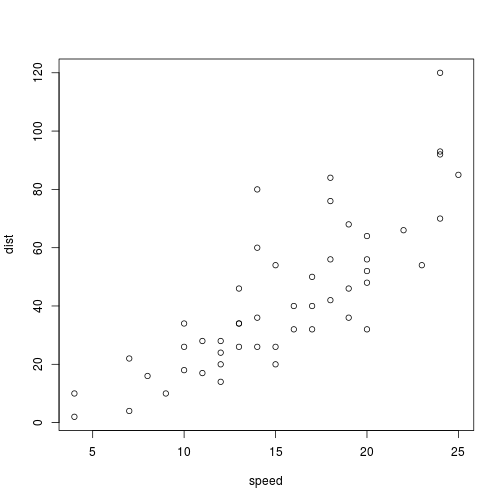
\includegraphics{micro_lunch_160301_files/figure-beamer/unnamed-chunk-2-1.pdf}

Simply receiving a letter had a sizeable initial impact which tapered
and dissipated with time

\end{frame}

\begin{frame}{Results: Main Treatments -- Participation}

\includegraphics{micro_lunch_160301_files/figure-beamer/EVER_PAID_7-1.pdf}

Deterrence-oriented treatments (Lien, Sheriff) effective, with some
catch-up; others, not so much.

\end{frame}

\begin{frame}{Results: Main Treatments -- Intensive Margin}

\includegraphics{micro_lunch_160301_files/figure-beamer/TOTAL_PAID_7-1.pdf}

No significant effect on \emph{amount} paid.

\end{frame}

\begin{frame}{Results: Heterogeneity by Owner Occupancy (I)}

\begin{table}[ht]
\centering
\begin{tabular}{lrr}
  \hline
Treatment & Non-Owner-Occ. & Owner-Occ. \\ 
  \hline
Control & 72 & 76 \\ 
  Amenities & 73 & 73 \\ 
  Moral & 74 & 74 \\ 
  Duty & 75 & 76 \\ 
  Peer & 73 & 76 \\ 
  Lien & 76 & 78 \\ 
  Sheriff & 78 & 77 \\ 
   \hline
\end{tabular}
\caption{Owner Occupancy Effect (Property-Level, Unique Owners)} 
\label{table:delta_by_owner_occ_unq}
\end{table}

\end{frame}

\begin{frame}{Results: Heterogeneity by Owner Occupancy (II)}

\begin{table}[ht]
\centering
\begin{tabular}{lrr}
  \hline
Treatment & Non-Owner-Occ. & Owner-Occ. \\ 
  \hline
Control & 80 & 88 \\ 
  Amenities & 77 & 80 \\ 
  Moral & 82 & 86 \\ 
  Duty & 80 & 86 \\ 
  Peer & 80 & 79 \\ 
  Lien & 82 & 90 \\ 
  Sheriff & 78 & 87 \\ 
   \hline
\end{tabular}
\caption{Owner Occupancy Effect (Property-Level, Multiple Owners)} 
\label{table:delta_by_owner_occ_mlt}
\end{table}

\end{frame}

\begin{frame}{Results: Letter-size Experiment}

\includegraphics{micro_lunch_160301_files/figure-beamer/EVER_PAID_2-1.pdf}

No discernible difference in uptake conditional on size of envelope
received.

\end{frame}

\begin{frame}{Results: Marginal Letter Receipt}

\includegraphics{micro_lunch_160301_files/figure-beamer/MARGINAL_LETTER-1.pdf}

Quantity of mail received has a marginal effect on participation.

\end{frame}

\begin{frame}{Results: Geographic Heterogeneity}

\includegraphics{micro_lunch_160301_files/figure-beamer/GEO_JULY-1.pdf}

Strong \emph{negative} effects in the Northeast early on.

\end{frame}

\begin{frame}{Results: Geographic Heterogeneity}

\includegraphics{micro_lunch_160301_files/figure-beamer/GEO_DECEMBER-1.pdf}

Mediation of negative effects in the Northeast, but effects crop up in
Center City.

\end{frame}

\begin{frame}{Results: Payment Agreements}

\includegraphics{micro_lunch_160301_files/figure-beamer/PAYMENT_AGREEMENT_7-1.pdf}

Differentiation of Sheriff vs.~Lien threat -- entrance into payment
agreements with DoR.

\end{frame}

\begin{frame}{Conclusion}

\begin{itemize}
\item
  Well-designed letters can have a noteworthy impact on the behavior of
  tax noncompliers at very low cost

  \begin{itemize}
  \item
    Total resources devoted to the project estimated at around \$30,000
    (including \$15,000 spent learning that large-format envelopes have
    little effect)
  \item
    Point estimate (not significant) of total returns to the experiment
    as a whole are around \$500,000
  \end{itemize}
\item
  The simple act of notification has a measurable impact on behavior,
  but, crucially, this effect appears to be ephemeral

  \begin{itemize}
  \tightlist
  \item
    Could still be a useful policy tool -- stems flow to (costly)
    subcontracted collections agencies
  \end{itemize}
\item
  Letters designed as \emph{tangible} threats can deliver a more
  sustained return

  \begin{itemize}
  \tightlist
  \item
    Localization, specificity breed credibility
  \end{itemize}
\end{itemize}

\end{frame}

\end{document}
